\documentclass[leqno]{article}
% Shared QBT/Soln pack preamble for resources.danieljsmith.org.
\usepackage{graphicx}
\usepackage{dsfont}
\usepackage{mathtools}
\usepackage{amssymb}
\usepackage{amsmath}
\usepackage{amsthm}
\usepackage{float}
\usepackage{ragged2e}
\usepackage{tensor}
\usepackage{fancyhdr}
\usepackage{empheq}
\usepackage[most]{tcolorbox}
\usepackage{enumitem}
\usepackage{dirtytalk}
\usepackage{marginnote}
\usepackage{microtype}
\usepackage[
  a4paper,
  left=0.8in,
  right=1in,
  top=1in,
  bottom=0.5in,
  headheight=14pt,
  headsep=0.4in
]{geometry}
\setlength{\parindent}{0cm}

% TikZ / PGFPlots
\usepackage{pgfplots}
\pgfplotsset{compat=1.18}
\usepgfplotslibrary{fillbetween, polar}
\usetikzlibrary{calc, positioning}
\usetikzlibrary{angles, quotes}
\usetikzlibrary{arrows.meta}
\usetikzlibrary{decorations.pathreplacing, decorations.markings}
\usetikzlibrary{patterns}
\usetikzlibrary{intersections}

% Links and contents
\usepackage[colorlinks=true,linkcolor=black,citecolor=magenta,urlcolor=black]{hyperref}%
\urlstyle{same}

% Pack macros
\RenewDocumentCommand{\marks}{o m}{%
  \IfValueTF{#1}%
    {\marginnote{\raggedright\textbf{[#2]}}[#1]}%
    {\marginnote{\raggedright\textbf{[#2]}}}%
}

\newcommand{\vspacerule}[2]{%
  \par\vspace*{#1}%
  \noindent\hrulefill\par
  \vspace*{#2}%
}

\definecolor{scarlet}{RGB}{205, 40, 75}

% Worked-solution box, adapted from the TMUA worked-solutions box. A white breakable box with a left scarlet rule and no surrounding
% frame or tint. A part that breaks fills the rest of its page, so the rule
% runs to the bottom margin; the unbroken or last part ends in a short
% horizontal foot rule so a solution visibly stops. Unlike the TMUA box there
% is no answer label and no extra \parskip: these solutions mix \\ line breaks
% with blank lines, so paragraph skips would make the spacing uneven. The box
% does not grow to the left, so the rule sits at the text edge; growing to the
% right keeps the usable line width close to the old tcolorbox Solution box.
\newtcolorbox{djsSolution}{%
  enhanced, breakable, frame hidden, sharp corners, colback=white,
  height fixed for=first and middle, height fill,
  extras unbroken and last={natural height},
  borderline west={2.2pt}{0pt}{scarlet},
  left=11pt, right=0pt, top=5pt, bottom=13pt,
  before skip=13pt, after skip=4pt,
  grow to right by=10mm,
  overlay unbroken and last={%
    \fill[scarlet] (frame.south west)
      rectangle ([xshift=3.5cm, yshift=2.2pt]frame.south west);},
  before upper={{\color{scarlet}\bfseries Solution}\par\vspace{4pt}}}

% Optional smaller figure inside a solution box. \scalebox shrinks node text
% with the drawing. Not applied to existing figures.
\newcommand{\SolnFigureScale}{0.85}
\newsavebox{\djsSolnFigureBox}
\newenvironment{djsSolutionFigure}
  {\par\vspace{4pt}\begin{center}\begin{lrbox}{\djsSolnFigureBox}}
  {\end{lrbox}\scalebox{\SolnFigureScale}{\usebox{\djsSolnFigureBox}}%
   \end{center}\vspace{2pt}\par}

\newcommand{\cxl}[2]{%
  \tikz[baseline=(X.base)]{%
    \node[inner sep=0pt, outer sep=0pt, text=#1] (X) {$#2$};
    \draw[#1, line width=0.4pt] (X.south west)--(X.north east);
  }%
}

% Page-style hook run at the contents page and each question's opening page.
% A no-op for QBT packs; \djsSolnHeader points it at the fancy header.
\newcommand{\djsQuestionPageStyle}{}

\newcommand{\questionitem}{%
  \djsQuestionPageStyle
  \item\phantomsection
  \addcontentsline{toc}{section}{Question \number\value{enumi}}%
}

\renewcommand{\contentsname}{Questions}

\newcommand{\djsPackHeader}[1]{%
  \pagestyle{fancy}%
  \fancyhead{}%
  \fancyfoot{}%
  \renewcommand{\headrulewidth}{0.9pt}%
  \lhead{#1}%
  \chead{}%
  \rhead{\href{https://danieljsmith.org}{danieljsmith.org}}%
}

\newcommand{\djsQbtHeader}[1]{%
  \djsPackHeader{#1}%
}

% Solutions packs show the header only on the contents page and each
% question's opening page, so it never appears part-way through a solution.
% \thispagestyle marks the next page shipped out, which is the question's
% page because every solution question starts after a \newpage.
\newcommand{\djsSolnHeader}[1]{%
  \djsPackHeader{\textit{Solutions} - #1}%
  \pagestyle{empty}%
  \renewcommand{\djsQuestionPageStyle}{\thispagestyle{fancy}}%
}

\newcommand{\djsFrontMatter}{%
  \djsQuestionPageStyle
  \vspace*{20pt}%
  \tableofcontents
  \newpage
}


\djsSolnHeader{Centre of Mass of Polygonal Laminae}

\begin{document}
\djsFrontMatter
\begin{enumerate}[
  label=\textbf{\arabic*.},
  leftmargin=*,
  topsep=0pt,
  partopsep=0pt,
  parsep=0pt
]

% ---- Question 1 ----
\questionitem
% [Source: _QBT___Solns__Centre_of_Mass_of_Polygonal_Laminae, Q1]

\begin{figure}[H]
    \centering
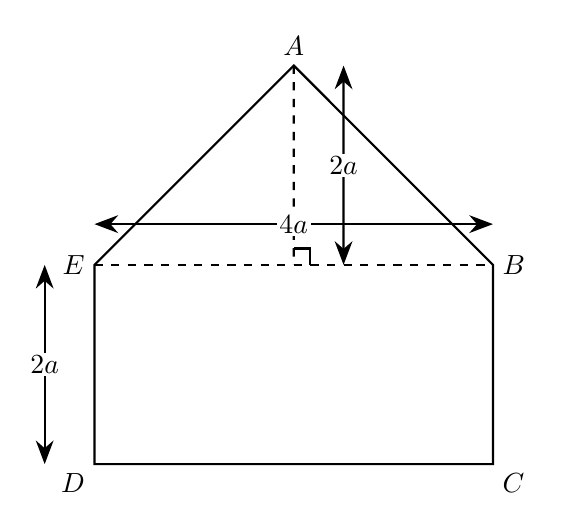
\begin{tikzpicture}[scale=1.15]
\def\a{1.1}
\coordinate (D) at (0,0);
\coordinate (C) at ({4*\a},0);
\coordinate (E) at (0,{2*\a});
\coordinate (B) at ({4*\a},{2*\a});
\coordinate (M) at ($(E)!0.5!(B)$);
\coordinate (A) at ($(M)+(0,{2*\a})$);

\draw[thick] (A) -- (B) -- (C) -- (D) -- (E) -- cycle;
\draw[dashed, thick] (E) -- (B);
\draw[dashed, thick] (A) -- (M);
\draw[thick] ($(M)+(0,0.18)$) -- ($(M)+(0.18,0.18)$) -- ($(M)+(0.18,0)$);

\draw[{Stealth[length=3mm]}-{Stealth[length=3mm]}, thick]
    ($(E)+(0,0.45)$) -- node[midway, fill=white, inner sep=1pt] {$4a$} ($(B)+(0,0.45)$);
\draw[{Stealth[length=3mm]}-{Stealth[length=3mm]}, thick]
    ($(D)+(-0.55,0)$) -- node[midway, fill=white, inner sep=1pt] {$2a$} ($(E)+(-0.55,0)$);
\draw[{Stealth[length=3mm]}-{Stealth[length=3mm]}, thick]
    ($(M)+(0.55,0)$) -- node[midway, fill=white, inner sep=1pt] {$2a$} ($(A)+(0.55,0)$);

\node[above] at (A) {$A$};
\node[right] at (B) {$B$};
\node[below right] at (C) {$C$};
\node[below left] at (D) {$D$};
\node[left] at (E) {$E$};
\end{tikzpicture}
\end{figure}


A uniform plane lamina is in the shape of the pentagon $ABCDE$, as shown shaded in the diagram above. \\
\begin{itemize}
  \item $BCDE$ is a rectangle
  \item $BE=4a$ and $DE=2a$
  \item triangle $ABE$ is isosceles with perpendicular height $2a$
\end{itemize}
\begin{enumerate}[label=\textbf{(\alph*)}]
  \item Show that the distance of the centre of mass of the lamina from $CD$ is $\dfrac{14a}{9}$. \marks{5} \\
\end{enumerate}
The mass of the lamina is $M$. \\

The lamina is suspended by two light vertical strings, one attached to the lamina at $D$ and the other attached to the lamina at $E$. \\

The lamina hangs freely in equilibrium, with $DE$ horizontal. \\
\begin{enumerate}[label=\textbf{(\alph*)}, resume]
  \item Using part (a), find, in terms of $M$ and $g$, the tension in the string attached at $E$. \marks{2} \\
\end{enumerate}

\vspace*{10pt}

\begin{tcolorbox}[colback=white, colframe=scarlet, title={\textbf{Solution}}, breakable, grow to left by=6mm, grow to right by=10mm]
\begin{enumerate}[label=\textbf{(\alph*)}, start=1]
  \item Split the lamina into rectangle $BCDE$ and triangle $ABE$.

Because the density is constant and the materials are the same, we can use areas as weights.

Let $\bar y$ be the distance of the centre of mass from $CD$.

For rectangle $BCDE$,
\[
\text{area}=BE\times DE=4a\times 2a=8a^2
\]
Its centre of mass is halfway up the rectangle, so its distance from $CD$ is
\[
a
\]

For triangle $ABE$,
\[
\text{area}=\frac12\times 4a\times 2a=4a^2
\]
The centre of mass of a triangle is $\frac13$ of the perpendicular height from the base.
So its distance above $BE$ is
\[
\frac13(2a)=\frac{2a}{3}
\]
Hence its distance from $CD$ is
\[
2a+\frac{2a}{3}=\frac{8a}{3}
\]

Now use moments of area about $CD$:
\begin{align*}
(8a^2+4a^2)\bar y&=8a^2(a)+4a^2\left(\frac{8a}{3}\right)\\
12a^2\bar y&=8a^3+\frac{32a^3}{3}\\
12a^2\bar y&=\frac{56a^3}{3}\\
\bar y&=\frac{56a^3}{36a^2}=\frac{14a}{9}
\end{align*}
So the distance of the centre of mass from $CD$ is $\dfrac{14a}{9}$.

  \item When the lamina hangs with $DE$ horizontal, the line $CD$ is vertical through $D$.
So, from part (a), the centre of mass is horizontally $\dfrac{14a}{9}$ from $D$.

Also, $DE=2a$, so the string at $E$ acts at a horizontal distance $2a$ from $D$.

Taking moments about $D$:
\[
T_E(2a)=Mg\left(\frac{14a}{9}\right)
\]
Hence
\[
T_E=\frac{Mg\left(\frac{14a}{9}\right)}{2a}=\frac{7Mg}{9}
\]
So the tension in the string attached at $E$ is $\dfrac{7Mg}{9}$.
\end{enumerate}
\end{tcolorbox}


\newpage

% ---- Question 2 ----
\questionitem
% [Source: _QBT___Solns__Centre_of_Mass_of_Polygonal_Laminae, Q2]

\begin{figure}[H]
    \centering
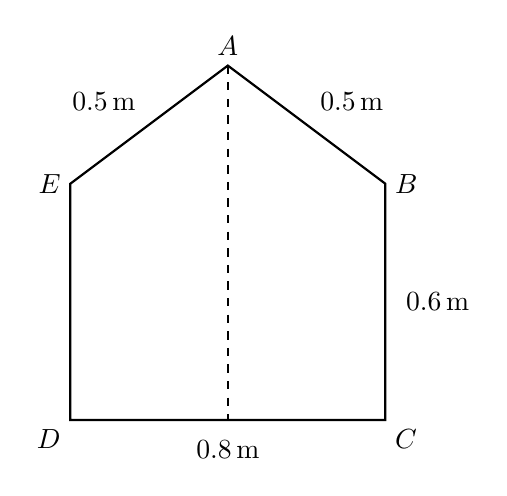
\begin{tikzpicture}[scale=5]
\def\w{0.8}
\def\h{0.6}
\def\roofside{0.5}
\pgfmathsetmacro{\halfw}{\w/2}
\pgfmathsetmacro{\roofh}{sqrt(\roofside*\roofside-\halfw*\halfw)}

\coordinate (D) at (-\halfw,0);
\coordinate (C) at (\halfw,0);
\coordinate (E) at (-\halfw,\h);
\coordinate (B) at (\halfw,\h);
\coordinate (A) at (0,{\h+\roofh});
\coordinate (M) at ($(C)!0.5!(D)$);

\draw[thick] (A) -- (B) -- (C) -- (D) -- (E) -- cycle;
\draw[dashed, thick] (A) -- (M);

\node[above] at (A) {$A$};
\node[right] at (B) {$B$};
\node[below right] at (C) {$C$};
\node[below left] at (D) {$D$};
\node[left] at (E) {$E$};

\node[above right=2pt] at ($(A)!0.5!(B)$) {$0.5\,\mathrm{m}$};
\node[above left=2pt] at ($(A)!0.5!(E)$) {$0.5\,\mathrm{m}$};
\node[right=4pt] at ($(B)!0.5!(C)$) {$0.6\,\mathrm{m}$};
\node[below=4pt] at ($(C)!0.5!(D)$) {$0.8\,\mathrm{m}$};
\end{tikzpicture}
\end{figure}


$ABCDE$ is a uniform lamina formed by joining an isosceles triangle $ABE$ to the top of a rectangle $BCDE$, where $AB=AE=0.5\,\mathrm{m}$, $BC=DE=0.6\,\mathrm{m}$ and $CD=BE=0.8\,\mathrm{m}$, as shown in the diagram. The centre of mass of the lamina is $G$. \\
\begin{enumerate}[label=\textbf{(\alph*)}]
  \item Explain why $G$ lies on the dashed line. \marks{1} \\
  \item Show that the perpendicular distance of $G$ from $CD$ is $0.38\,\mathrm{m}$. \marks{4} \\
\end{enumerate}
The lamina is freely suspended from the point $B$. \\
\begin{enumerate}[label=\textbf{(\alph*)}, resume]
  \item Determine the acute angle that $CD$ makes with the horizontal, stating which of $C$ or $D$ is higher. \marks{4} \\
\end{enumerate}

\vspace*{10pt}

\begin{tcolorbox}[colback=white, colframe=scarlet, title={\textbf{Solution}}, breakable, grow to left by=6mm, grow to right by=10mm]
\begin{enumerate}[label=\textbf{(\alph*)}, start=1]
  \item The lamina is uniform and symmetric about the dashed line \(AM\). Therefore its centre of mass must lie on this line, so \(G\) lies on the dashed line of symmetry.

  \item Let \(M\) be the midpoint of \(CD\), so \(AM\) is the line of symmetry.

For rectangle \(BCDE\),
\[
\text{area} = 0.8 \times 0.6 = 0.48
\]
and its centre is halfway up the rectangle, so it is
\[
0.3\,\mathrm{m}
\]
above \(CD\).

For triangle \(ABE\), the base is \(BE=0.8\,\mathrm{m}\), so
\[
BM=EM=0.4\,\mathrm{m}
\]
Hence its height is
\begin{align*}
AM &= \sqrt{AB^2-BM^2} \\
   &= \sqrt{0.5^2-0.4^2} \\
   &= \sqrt{0.25-0.16} \\
   &= 0.3\,\mathrm{m}
\end{align*}
So the area of the triangle is
\[
\frac12 \times 0.8 \times 0.3 = 0.12
\]

The centre of mass of a triangle is one-third of the height from its base, so the triangle's centre of mass is
\[
0.6 + \frac{0.3}{3} = 0.7\,\mathrm{m}
\]
above \(CD\).

Because the density is constant and the materials are the same, we can use areas as weights:
\[
Ay = A_1y_1 + A_2y_2
\]
So
\begin{align*}
(0.48+0.12)y &= 0.48(0.3)+0.12(0.7) \\
0.6y &= 0.144+0.084 \\
0.6y &= 0.228 \\
y &= 0.38
\end{align*}
So the perpendicular distance of \(G\) from \(CD\) is \(0.38\,\mathrm{m}\).

  \item From part (b), \(G\) is \(0.38\,\mathrm{m}\) above \(CD\), while \(B\) is \(0.6\,\mathrm{m}\) above \(CD\). So \(G\) is
\[
0.6-0.38=0.22\,\mathrm{m}
\]
below \(B\).

Also, since \(G\) lies on the line of symmetry \(AM\), its horizontal distance from \(B\) is half the width of the rectangle:
\[
BM=\frac{CD}{2}=0.4\,\mathrm{m}
\]

When the lamina is freely suspended from \(B\), the centre of mass \(G\) hangs vertically below \(B\). Therefore the lamina must rotate through an angle \(\theta\) where
\begin{align*}
\tan\theta &= \frac{\text{horizontal distance of }G\text{ from }B}{\text{vertical distance of }G\text{ below }B} \\
&= \frac{0.4}{0.22} \\
&= \frac{20}{11}
\end{align*}
Hence
\[
\theta = \tan^{-1}\!\left(\frac{20}{11}\right) \approx 61.2^\circ
\]

Since \(G\) is to the left of \(B\), the lamina rotates clockwise, so \(D\) is higher than \(C\).

So the acute angle that \(CD\) makes with the horizontal is
\[
\tan^{-1}\!\left(\frac{20}{11}\right) \approx 61.2^\circ
\]
with \(D\) higher than \(C\).
\end{enumerate}
\end{tcolorbox}


\newpage

% ---- Question 3 ----
\questionitem
% [Source: _QBT___Solns__Centre_of_Mass_of_Polygonal_Laminae, Q3]

\begin{figure}[H]
    \centering
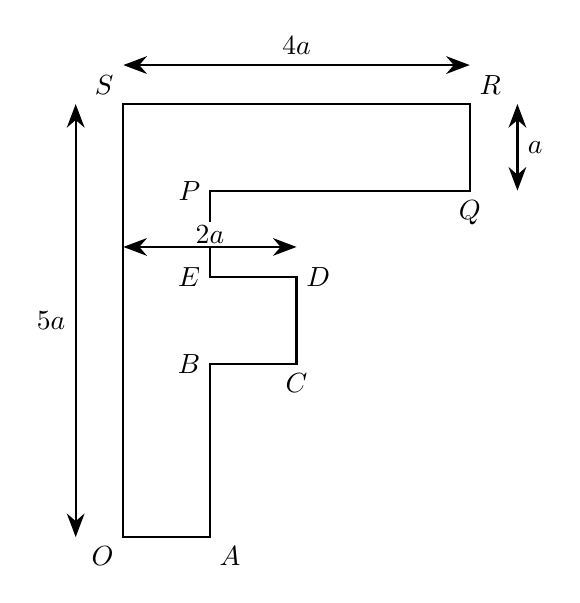
\begin{tikzpicture}[scale=1.0]
\def\a{1.1}

\coordinate (O) at (0,0);
\coordinate (A) at (\a,0);
\coordinate (B) at (\a,{2*\a});
\coordinate (C) at ({2*\a},{2*\a});
\coordinate (D) at ({2*\a},{3*\a});
\coordinate (E) at (\a,{3*\a});
\coordinate (P) at (\a,{4*\a});
\coordinate (Q) at ({4*\a},{4*\a});
\coordinate (R) at ({4*\a},{5*\a});
\coordinate (S) at (0,{5*\a});

\coordinate (V1) at ({-0.55*\a},0);
\coordinate (V2) at ({-0.55*\a},{5*\a});
\coordinate (H1) at (0,{5.45*\a});
\coordinate (H2) at ({4*\a},{5.45*\a});
\coordinate (M1) at (0,{3.35*\a});
\coordinate (M2) at ({2*\a},{3.35*\a});
\coordinate (T1) at ({4.55*\a},{4*\a});
\coordinate (T2) at ({4.55*\a},{5*\a});

\draw[thick] (O) -- (A) -- (B) -- (C) -- (D) -- (E) -- (P) -- (Q) -- (R) -- (S) -- cycle;

\draw[{Stealth[length=3mm]}-{Stealth[length=3mm]}, thick] (V1) -- (V2) node[midway,left] {$5a$};
\draw[{Stealth[length=3mm]}-{Stealth[length=3mm]}, thick] (H1) -- (H2) node[midway,above] {$4a$};
\draw[{Stealth[length=3mm]}-{Stealth[length=3mm]}, thick] (M1) -- (M2) node[midway,above,fill=white,inner sep=1pt] {$2a$};
\draw[{Stealth[length=3mm]}-{Stealth[length=3mm]}, thick] (T1) -- (T2) node[midway,right] {$a$};

\node[below left] at (O) {$O$};
\node[below right] at (A) {$A$};
\node[left] at (B) {$B$};
\node[below] at (C) {$C$};
\node[right] at (D) {$D$};
\node[left] at (E) {$E$};
\node[left] at (P) {$P$};
\node[below] at (Q) {$Q$};
\node[above right] at (R) {$R$};
\node[above left] at (S) {$S$};
\end{tikzpicture}
\end{figure}


A letter $F$ from a shop sign is modelled as a uniform plane lamina in the shape shown in the diagram above. \\

The left-hand vertical strip has width $a$ and height $5a$. The top horizontal strip has length $4a$ and thickness $a$. The middle horizontal strip has length $2a$ and thickness $a$. \\

Using the model, \\
\begin{enumerate}[label=\textbf{(\alph*)}]
  \item find, in terms of $a$, the distance of the centre of mass of the letter $F$, from
  \begin{enumerate}[label=(\roman*)]
    \item $OS$
    \item $OA$
  \end{enumerate}
  \marks{6}
\end{enumerate}
The letter $F$ is freely suspended from $O$ and hangs in equilibrium. The angle between $OS$ and the downward vertical is $\alpha$. \\

Using the model, \\
\begin{enumerate}[label=\textbf{(\alph*)}, resume]
  \item find the exact value of $\tan\alpha$. \marks{2} \\
\end{enumerate}

\vspace*{10pt}

\begin{tcolorbox}[colback=white, colframe=scarlet, title={\textbf{Solution}}, breakable, grow to left by=6mm, grow to right by=10mm]
\begin{enumerate}[label=\textbf{(\alph*)}, start=1]
  \item Take \(O\) as the origin, with \(OA\) as the \(x\)-axis and \(OS\) as the \(y\)-axis.

  To avoid overlap, split the letter \(F\) into three rectangles:
\[
\begingroup
\renewcommand{\arraystretch}{2.2}
\begin{array}{c|c|c|c}
\text{Part} & \text{Area} & x\text{-coordinate of centre} & y\text{-coordinate of centre} \\
\hline
\text{vertical strip} & 5a^2 & \dfrac{a}{2} & \dfrac{5a}{2} \\
\text{top extension} & 3a^2 & \dfrac{5a}{2} & \dfrac{9a}{2} \\
\text{middle extension} & a^2 & \dfrac{3a}{2} & \dfrac{5a}{2}
\end{array}
\endgroup
\]

  Because the density is constant and the material is the same, we can use areas as weights.

  The total area is
  \[
  A=5a^2+3a^2+a^2=9a^2
  \]

  \begin{enumerate}[label=\textbf{(\roman*)}, start=1]
    \item If the centre of mass is \((\bar x,\bar y)\), then the distance from \(OS\) is \(\bar x\).

    \begin{align*}
    A\bar x
    &=5a^2\left(\frac{a}{2}\right)+3a^2\left(\frac{5a}{2}\right)+a^2\left(\frac{3a}{2}\right)\\
    &=\frac{5a^3}{2}+\frac{15a^3}{2}+\frac{3a^3}{2}\\
    &=\frac{23a^3}{2}
    \end{align*}

    So
    \[
    \bar x=\frac{\frac{23a^3}{2}}{9a^2}=\frac{23a}{18}
    \]

    Hence the distance of the centre of mass from \(OS\) is \(\dfrac{23a}{18}\).

    \item The distance from \(OA\) is \(\bar y\).

    \begin{align*}
    A\bar y
    &=5a^2\left(\frac{5a}{2}\right)+3a^2\left(\frac{9a}{2}\right)+a^2\left(\frac{5a}{2}\right)\\
    &=\frac{25a^3}{2}+\frac{27a^3}{2}+\frac{5a^3}{2}\\
    &=\frac{57a^3}{2}
    \end{align*}

    So
    \[
    \bar y=\frac{\frac{57a^3}{2}}{9a^2}=\frac{57a}{18}=\frac{19a}{6}
    \]

    Hence the distance of the centre of mass from \(OA\) is \(\dfrac{19a}{6}\).
  \end{enumerate}

  \item Let the centre of mass be \(G\).

  When the lamina is freely suspended from \(O\), it hangs with \(G\) vertically below \(O\). So the downward vertical is the line \(OG\).

  Therefore \(\alpha\) is the angle between \(OS\) and \(OG\). Using the coordinates of \(G\) found in part (a),
  \[
  \tan\alpha=\frac{\text{distance of }G\text{ from }OS}{\text{distance of }G\text{ from }OA}
  =\frac{\bar x}{\bar y}
  \]

  Hence
  \begin{align*}
  \tan\alpha
  &=\frac{\frac{23a}{18}}{\frac{19a}{6}}\\
  &=\frac{23a}{18}\times\frac{6}{19a}\\
  &=\frac{23}{57}
  \end{align*}

  So the exact value is \(\tan\alpha=\dfrac{23}{57}\).
\end{enumerate}
\end{tcolorbox}


\newpage

% ---- Question 4 ----
\questionitem
% [Source: _QBT___Solns__Centre_of_Mass_of_Polygonal_Laminae, Q4]

\begin{figure}[H]
    \centering
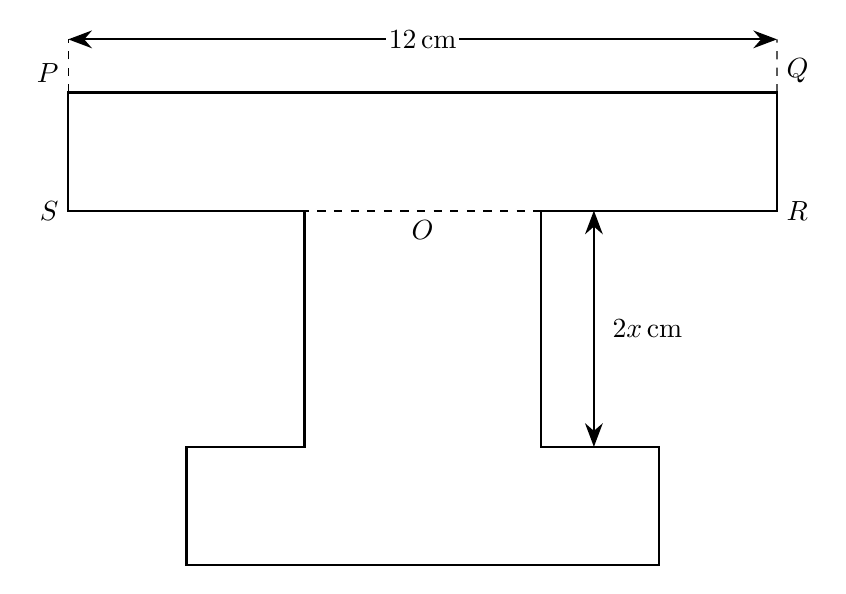
\begin{tikzpicture}[scale=0.75]
\def\Wtop{12}
\def\Hbar{2}
\def\Wstem{4}
\def\Wbot{8}
\def\Hbot{2}
\def\xshown{2}
\def\topoff{0.9}
\def\sideoff{0.9}
\pgfmathsetmacro{\Hstem}{2*\xshown}
\pgfmathsetmacro{\yref}{\Hbot+\Hstem}
\pgfmathsetmacro{\ytop}{\yref+\Hbar}
\pgfmathsetmacro{\xleftstem}{(\Wtop-\Wstem)/2}
\pgfmathsetmacro{\xrightstem}{(\Wtop+\Wstem)/2}
\pgfmathsetmacro{\xleftbot}{(\Wtop-\Wbot)/2}
\pgfmathsetmacro{\xrightbot}{(\Wtop+\Wbot)/2}

\coordinate (P) at (0,\ytop);
\coordinate (Q) at (\Wtop,\ytop);
\coordinate (R) at (\Wtop,\yref);
\coordinate (S) at (0,\yref);
\coordinate (O) at ($(S)!0.5!(R)$);
\coordinate (A) at (\xleftstem,\yref);
\coordinate (B) at (\xrightstem,\yref);
\coordinate (C) at (\xrightstem,\Hbot);
\coordinate (D) at (\xleftstem,\Hbot);
\coordinate (E) at (\xleftbot,\Hbot);
\coordinate (F) at (\xrightbot,\Hbot);
\coordinate (G) at (\xrightbot,0);
\coordinate (H) at (\xleftbot,0);
\coordinate (Pdim) at ($(P)+(0,\topoff)$);
\coordinate (Qdim) at ($(Q)+(0,\topoff)$);
\coordinate (Bdim) at ($(B)+(\sideoff,0)$);
\coordinate (Cdim) at ($(C)+(\sideoff,0)$);

\draw[dashed, thick] (S) -- (R);

\draw[thick]
  (P) -- (Q) -- (R) -- (B) -- (C) -- (F) -- (G) -- (H) -- (E) -- (D) -- (A) -- (S) -- cycle;

\draw[dashed] (P) -- (Pdim);
\draw[dashed] (Q) -- (Qdim);
\draw[{Stealth[length=3mm]}-{Stealth[length=3mm]}, thick]
  (Pdim) -- node[midway, fill=white, inner sep=1pt] {$12\,\mathrm{cm}$} (Qdim);

\draw[dashed] (B) -- (Bdim);
\draw[dashed] (C) -- (Cdim);
\draw[{Stealth[length=3mm]}-{Stealth[length=3mm]}, thick]
  (Cdim) -- node[midway, right=3pt] {$2x\,\mathrm{cm}$} (Bdim);

\node[above left] at (P) {$P$};
\node[above right] at (Q) {$Q$};
\node[right] at (R) {$R$};
\node[left] at (S) {$S$};
\node[below] at (O) {$O$};
\end{tikzpicture}
\end{figure}


A template $T$ consists of a uniform plane lamina made from three rectangles, as shown in the diagram. The upper rectangle $PQRS$ has $PQ=12\,\mathrm{cm}$ and $PS=2\,\mathrm{cm}$. The point $O$ is the midpoint of $SR$. A rectangle of width $4\,\mathrm{cm}$ and height $2x\,\mathrm{cm}$ is attached centrally below $SR$, and a rectangle of width $8\,\mathrm{cm}$ and height $2\,\mathrm{cm}$ is attached centrally below this rectangle. The whole template is symmetrical about the line through $O$ perpendicular to $SR$, where $x>1$. \\
\begin{enumerate}[label=\textbf{(\alph*)}]
  \item Show that the centre of mass of $T$ is a distance
  \[
  \dfrac{x^2+4x-1}{x+5}\,\mathrm{cm}
  \]
  below $SR$. \marks{7} \\
\end{enumerate}
The template $T$ is freely suspended from the point $P$ and hangs in equilibrium. \\

Given that $x=2$ and that $\theta$ is the angle that $PQ$ makes with the horizontal, \\
\begin{enumerate}[label=\textbf{(\alph*)}, resume]
  \item show that
  \[
  \tan\theta=\dfrac{42}{25}
  \]
  \marks[-20pt]{4}
\end{enumerate}

\vspace*{10pt}

\begin{tcolorbox}[colback=white, colframe=scarlet, title={\textbf{Solution}}, breakable, grow to left by=6mm, grow to right by=10mm]
\begin{enumerate}[label=\textbf{(\alph*)}, start=1]
  \item Let the centre of mass be $G$.

Since the template is symmetrical about the line through $O$ perpendicular to $SR$, the point $G$ lies on this line.

Take distances from $SR$, positive downwards.

Because the density is constant and the materials are the same, we can use areas as weights in
\[
A\bar y=A_1y_1+A_2y_2+A_3y_3.
\]

For the three rectangles:
\begin{align*}
\text{upper rectangle: }&A_1=12\times 2=24, &&y_1=-1 \\
\text{middle rectangle: }&A_2=4\times 2x=8x, &&y_2=x \\
\text{lower rectangle: }&A_3=8\times 2=16, &&y_3=2x+1
\end{align*}

So
\begin{align*}
(24+8x+16)\bar y&=24(-1)+8x(x)+16(2x+1)\\
&=-24+8x^2+32x+16\\
&=8x^2+32x-8\\
&=8(x^2+4x-1).
\end{align*}

Also,
\[
24+8x+16=8x+40=8(x+5).
\]

Hence
\[
\bar y=\frac{8(x^2+4x-1)}{8(x+5)}=\frac{x^2+4x-1}{x+5}.
\]

Since $x>1$, this value is positive, so $G$ is below $SR$.

Therefore the centre of mass is
\[
\frac{x^2+4x-1}{x+5}\,\mathrm{cm}
\]
below $SR$.

  \item From part (a), when $x=2$,
\[
OG=\frac{2^2+4(2)-1}{2+5}=\frac{11}{7}\,\mathrm{cm}.
\]

So $G$ is $\frac{11}{7}$ cm below $SR$ on the line of symmetry through $O$.

The horizontal distance from $P$ to this line is half of $PQ$, so
\[
\text{horizontal distance }=\frac{12}{2}=6\,\mathrm{cm}.
\]

The vertical distance from $P$ down to $G$ is
\[
PS+OG=2+\frac{11}{7}=\frac{25}{7}\,\mathrm{cm}.
\]

Let $\alpha$ be the angle between $PQ$ and $PG$. Then
\[
\tan\alpha=\frac{25/7}{6}=\frac{25}{42}.
\]

When the template hangs freely from $P$, the centre of mass is vertically below $P$, so $PG$ is vertical.
Hence $PQ$ makes an angle $\theta$ with the horizontal where
\[
\theta=90^\circ-\alpha.
\]

Therefore
\[
\tan\theta=\tan(90^\circ-\alpha)=\frac{1}{\tan\alpha}=\frac{42}{25}.
\]

So
\[
\tan\theta=\frac{42}{25}.
\]
\end{enumerate}
\end{tcolorbox}

\newpage

% ---- Question 5 ----
\questionitem
% [Source: _QBT___Solns__Centre_of_Mass_of_Polygonal_Laminae, Q5]

\begin{figure}[H]
    \centering
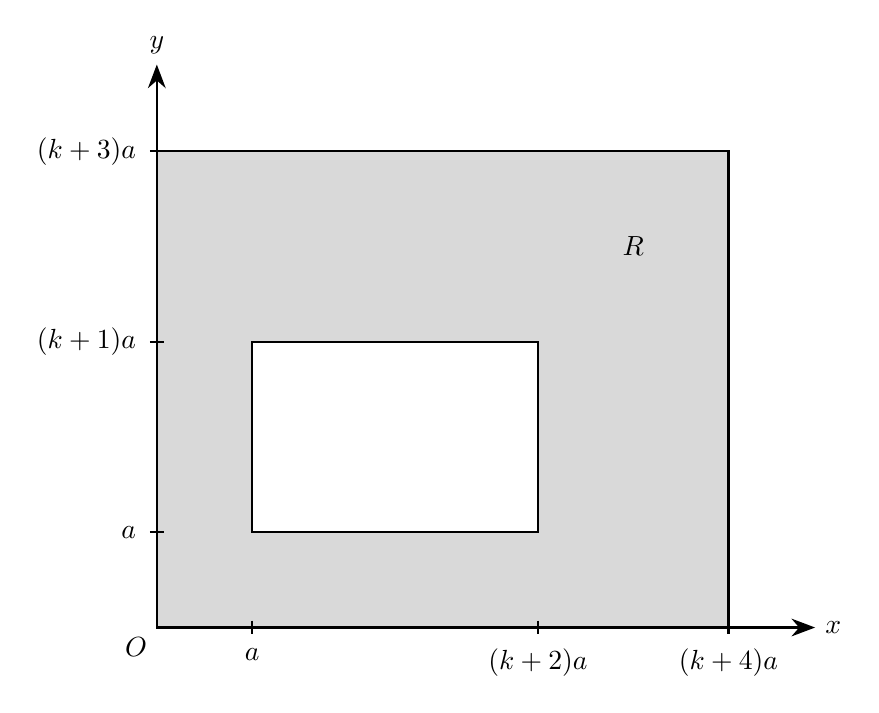
\begin{tikzpicture}[scale=1.1]
\def\alen{1.1}
\def\kval{2}
\pgfmathsetmacro{\xinnerL}{\alen}
\pgfmathsetmacro{\xinnerR}{(\kval+2)*\alen}
\pgfmathsetmacro{\xouter}{(\kval+4)*\alen}
\pgfmathsetmacro{\yinnerB}{\alen}
\pgfmathsetmacro{\yinnerT}{(\kval+1)*\alen}
\pgfmathsetmacro{\youter}{(\kval+3)*\alen}
\pgfmathsetmacro{\xmax}{\xouter+1.0}
\pgfmathsetmacro{\ymax}{\youter+1.0}

\coordinate (O) at (0,0);

\draw[-{Stealth[length=3mm]}, thick] (O) -- (\xmax,0) node[right] {$x$};
\draw[-{Stealth[length=3mm]}, thick] (O) -- (0,\ymax) node[above] {$y$};

\fill[gray!30, even odd rule] (0,0) rectangle (\xouter,\youter) (\xinnerL,\yinnerB) rectangle (\xinnerR,\yinnerT);
\draw[thick] (0,0) rectangle (\xouter,\youter);
\draw[thick] (\xinnerL,\yinnerB) rectangle (\xinnerR,\yinnerT);

\node[below left] at (O) {$O$};
\node at ({(\xinnerR+\xouter)/2},{(\yinnerT+\youter)/2}) {$R$};

\foreach \x in {\xinnerL,\xinnerR,\xouter} {
  \draw[thick] (\x,0.08) -- (\x,-0.08);
}

\foreach \y in {\yinnerB,\yinnerT,\youter} {
  \draw[thick] (-0.08,\y) -- (0.08,\y);
}

\node[below=4pt] at (\xinnerL,0) {$a$};
\node[below=4pt] at (\xinnerR,0) {$(k+2)a$};
\node[below=4pt] at (\xouter,0) {$(k+4)a$};

\node[left=4pt] at (0,\yinnerB) {$a$};
\node[left=4pt] at (0,\yinnerT) {$(k+1)a$};
\node[left=4pt] at (0,\youter) {$(k+3)a$};
\end{tikzpicture}
\end{figure}


A uniform lamina $R$ is bounded externally by the rectangle with vertices $(0,0)$, $((k+4)a,0)$, \\$((k+4)a,(k+3)a)$ and $(0,(k+3)a)$, where $k>0$.\\

A rectangular hole with vertices $(a,a)$, $((k+2)a,a)$, $((k+2)a,(k+1)a)$ and $(a,(k+1)a)$ is removed, as shown in the diagram. \\

Determine the range of values of $k$ for which the centre of mass of $R$ lies in the hole. \marks{10} \\

\vspace*{10pt}

\begin{tcolorbox}[colback=white, colframe=scarlet, title={\textbf{Solution}}, breakable, grow to left by=6mm, grow to right by=10mm]
Let the outer rectangle be $R_1$ and the rectangular hole be $R_2$.

Because the density is constant and the materials are the same, areas can be used as weights.

For $R_1$,
\[
A_1=(k+4)(k+3)a^2,
\qquad
\left(x_1,y_1\right)=\left(\frac{(k+4)a}{2},\frac{(k+3)a}{2}\right)
\]

For the hole $R_2$,
\[
A_2=\bigl((k+2)a-a\bigr)\bigl((k+1)a-a\bigr)=k(k+1)a^2
\]
and its centre is
\[
\left(x_2,y_2\right)=\left(\frac{a+(k+2)a}{2},\frac{a+(k+1)a}{2}\right)=\left(\frac{(k+3)a}{2},\frac{(k+2)a}{2}\right)
\]

So the area of the remaining lamina $R$ is
\[
A=A_1-A_2=\bigl((k+4)(k+3)-k(k+1)\bigr)a^2=6(k+2)a^2
\]

Using subtraction of moments,
\[
A\bar x=A_1x_1-A_2x_2,
\qquad
A\bar y=A_1y_1-A_2y_2
\]

Hence
\begin{align*}
\bar x
&=\frac{(k+4)(k+3)a^2\cdot \frac{(k+4)a}{2}-k(k+1)a^2\cdot \frac{(k+3)a}{2}}{6(k+2)a^2}\\[4pt]
&=\frac{a(k+3)\bigl((k+4)^2-k(k+1)\bigr)}{12(k+2)}\\[4pt]
&=\frac{a(k+3)(7k+16)}{12(k+2)}
\end{align*}

and
\begin{align*}
\bar y
&=\frac{(k+4)(k+3)a^2\cdot \frac{(k+3)a}{2}-k(k+1)a^2\cdot \frac{(k+2)a}{2}}{6(k+2)a^2}\\[4pt]
&=\frac{a\bigl((k+4)(k+3)^2-k(k+1)(k+2)\bigr)}{12(k+2)}\\[4pt]
&=\frac{a(7k^2+31k+36)}{12(k+2)}
\end{align*}

For the centre of mass to lie inside the hole, we need
\[
a<\bar x<(k+2)a,
\qquad
a<\bar y<(k+1)a
\]
Since $a>0$ and $k>0$, we can divide through by $a$.

First, for the $x$-coordinate,
\begin{align*}
\bar x>a
&\iff \frac{(k+3)(7k+16)}{12(k+2)}>1\\[4pt]
&\iff (k+3)(7k+16)>12(k+2)\\[4pt]
&\iff 7k^2+25k+24>0
\end{align*}
which is true for all $k>0$.

Also,
\begin{align*}
\bar x<(k+2)a
&\iff \frac{(k+3)(7k+16)}{12(k+2)}<k+2\\[4pt]
&\iff (k+3)(7k+16)<12(k+2)^2\\[4pt]
&\iff 5k^2+11k>0
\end{align*}
which is also true for all $k>0$.

Now for the $y$-coordinate,
\begin{align*}
\bar y>a
&\iff \frac{7k^2+31k+36}{12(k+2)}>1\\[4pt]
&\iff 7k^2+31k+36>12(k+2)\\[4pt]
&\iff 7k^2+19k+12>0
\end{align*}
which is true for all $k>0$.

Finally,
\begin{align*}
\bar y<(k+1)a
&\iff \frac{7k^2+31k+36}{12(k+2)}<k+1\\[4pt]
&\iff 7k^2+31k+36<12(k+2)(k+1)\\[4pt]
&\iff 5k^2+5k-12>0
\end{align*}

Solving $5k^2+5k-12=0$,
\[
k=\frac{-5\pm\sqrt{25+240}}{10}=\frac{-5\pm\sqrt{265}}{10}
\]
Since the quadratic opens upwards, $5k^2+5k-12>0$ when
\[
k<\frac{-5-\sqrt{265}}{10}
\quad\text{or}\quad
k>\frac{-5+\sqrt{265}}{10}
\]
But $k>0$, so the only possible range is
\[
k>\frac{\sqrt{265}-5}{10}
\]

Therefore the centre of mass of $R$ lies in the hole when
\[
\boxed{\;k>\frac{\sqrt{265}-5}{10}\;}\approx 1.13
\]
\end{tcolorbox}


\newpage

% ---- Question 6 ----
\questionitem
% [Source: _QBT___Solns__Centre_of_Mass_of_Polygonal_Laminae, Q6]

\begin{figure}[H]
    \centering
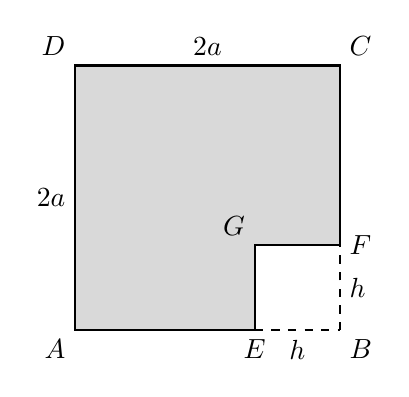
\begin{tikzpicture}[scale=1.2]
\def\aunit{1.4}
\def\hlen{0.9}
\pgfmathsetmacro{\side}{2*\aunit}

\coordinate (A) at (0,0);
\coordinate (B) at (\side,0);
\coordinate (C) at (\side,\side);
\coordinate (D) at (0,\side);
\coordinate (E) at ({\side-\hlen},0);
\coordinate (F) at (\side,\hlen);
\coordinate (G) at ({\side-\hlen},\hlen);

\fill[gray!30] (A) -- (E) -- (G) -- (F) -- (C) -- (D) -- cycle;
\draw[thick] (A) -- (E) -- (G) -- (F) -- (C) -- (D) -- cycle;
\draw[dashed, thick] (E) -- (B);
\draw[dashed, thick] (B) -- (F);

\node[below] at ($(E)!0.5!(B)$) {$h$};
\node[right] at ($(B)!0.5!(F)$) {$h$};
\node[above] at ($(D)!0.5!(C)$) {$2a$};
\node[left] at ($(A)!0.5!(D)$) {$2a$};

\node[below left] at (A) {$A$};
\node[below right] at (B) {$B$};
\node[above right] at (C) {$C$};
\node[above left] at (D) {$D$};
\node[below] at (E) {$E$};
\node[right] at (F) {$F$};
\node[above left] at (G) {$G$};
\end{tikzpicture}
\end{figure}


A uniform lamina is formed by removing the square $EBGF$ from a square lamina $ABCD$, where $AB=BC=CD=DA=2a$ and $EB=BF=h$, with $0<h<2a$ (see diagram). \\
\begin{enumerate}[label=\textbf{(\alph*)}]
  \item Find the distance of the centre of mass of the remaining lamina from $AD$ and from $AB$, giving your answers in terms of $a$ and $h$. \marks{5} \\
\end{enumerate}
The lamina is placed vertically on its edge $AE$ on a horizontal plane. \\
\begin{enumerate}[label=\textbf{(\alph*)}, resume]
  \item Find, in terms of $a$, the set of values of $h$ for which the lamina remains in equilibrium. \marks{3} \\
\end{enumerate}

\vspace*{10pt}

\begin{tcolorbox}[colback=white, colframe=scarlet, title={\textbf{Solution}}, breakable, grow to left by=6mm, grow to right by=10mm]
\begin{enumerate}[label=\textbf{(\alph*)}, start=1]
  \item Let the centre of mass of the remaining lamina be \((\bar x,\bar y)\), where \(\bar x\) is the distance from \(AD\) and \(\bar y\) is the distance from \(AB\).

Because the density is constant and the materials are the same:
\[
\text{area of }ABCD=4a^2, \qquad \text{centre }(a,a)
\]
\[
\text{area of removed square }EBGF=h^2, \qquad \text{centre }\left(2a-\frac h2,\frac h2\right)
\]
So the area of the remaining lamina is
\[
4a^2-h^2
\]
For the distance from \(AD\), use areas as weights:
\[
(4a^2-h^2)\bar x=4a^2(a)-h^2\left(2a-\frac h2\right)
\]
\begin{align*}
\bar x&=\frac{4a^3-2ah^2+\frac12h^3}{4a^2-h^2}\\
&=\frac{a(4a^2-h^2)-\frac12h^2(2a-h)}{(2a-h)(2a+h)}\\
&=a-\frac{h^2}{2(2a+h)}
\end{align*}
For the distance from \(AB\):
\[
(4a^2-h^2)\bar y=4a^2(a)-h^2\left(\frac h2\right)
\]
\begin{align*}
\bar y&=\frac{4a^3-\frac12h^3}{4a^2-h^2}\\
&=\frac{a(4a^2-h^2)+\frac12h^2(2a-h)}{(2a-h)(2a+h)}\\
&=a+\frac{h^2}{2(2a+h)}
\end{align*}
Therefore the centre of mass is at distance
\[
a-\frac{h^2}{2(2a+h)}
\]
from \(AD\), and at distance
\[
a+\frac{h^2}{2(2a+h)}
\]
from \(AB\)

  \item When the lamina is placed vertically on edge \(AE\), it will remain in equilibrium if the vertical line through the centre of mass meets the base \(AE\).

Now
\[
AE=AB-EB=2a-h
\]
In this position, the horizontal position of the centre of mass along the base is \(\bar x\). So we require
\[
0\le \bar x\le 2a-h
\]
Since \(\bar x>0\), it is enough to solve
\[
a-\frac{h^2}{2(2a+h)}\le 2a-h
\]
\begin{align*}
-h^2&\le 2(2a+h)(a-h)\\
-h^2&\le 4a^2-2ah-2h^2\\
h^2+2ah-4a^2&\le 0
\end{align*}
The roots of \(h^2+2ah-4a^2=0\) are
\[
h=\frac{-2a\pm\sqrt{4a^2+16a^2}}{2}=-a\pm a\sqrt5
\]
So
\[
-a(1+\sqrt5)\le h\le a(\sqrt5-1)
\]
Given that \(0<h<2a\), this reduces to
\[
0<h\le a(\sqrt5-1)
\]
Therefore the lamina remains in equilibrium for
\[
0<h\le a(\sqrt5-1)
\]
\end{enumerate}
\end{tcolorbox}


\newpage

% ---- Question 7 ----
\questionitem
% [Source: _QBT___Solns__Centre_of_Mass_of_Polygonal_Laminae, Q7]

\begin{figure}[H]
    \centering
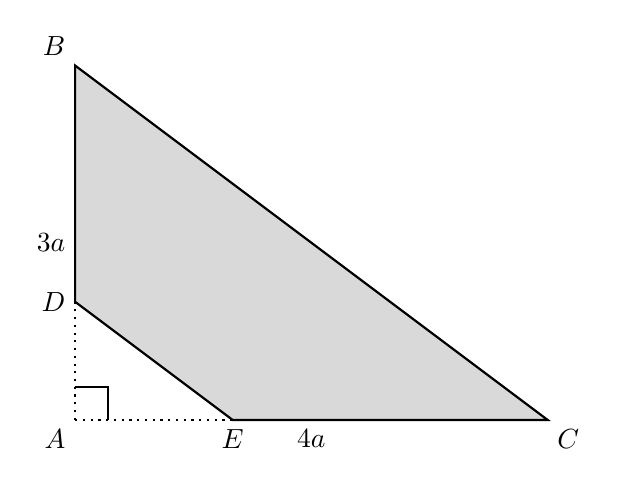
\begin{tikzpicture}[scale=1.5]
\def\xC{4}
\def\yB{3}
\def\kshown{3}
\pgfmathsetmacro{\t}{1/\kshown}

\coordinate (A) at (0,0);
\coordinate (B) at (0,\yB);
\coordinate (C) at (\xC,0);
\coordinate (D) at (0,{\yB*\t});
\coordinate (E) at ({\xC*\t},0);

\fill[gray!30] (D) -- (B) -- (C) -- (E) -- cycle;

\draw[thick] (D) -- (B) -- (C) -- (E) -- cycle;
\draw[dotted, thick] (A) -- (D);
\draw[dotted, thick] (A) -- (E);

\draw[thick] (0.28,0) -- (0.28,0.28) -- (0,0.28);

\node[below left] at (A) {$A$};
\node[above left] at (B) {$B$};
\node[below right] at (C) {$C$};
\node[left] at (D) {$D$};
\node[below] at (E) {$E$};
\node[left] at ($(A)!0.5!(B)$) {$3a$};
\node[below] at ($(A)!0.5!(C)$) {$4a$};
\end{tikzpicture}
\end{figure}


A uniform lamina is formed from the right-angled triangle $ABC$ by removing the triangle $ADE$, as shown in the diagram. The triangle $ABC$ has $AB=3a$, $AC=4a$ and $\angle BAC=90^\circ$. The point $D$ lies on $AB$ and satisfies $AD:AB=1:k$. The point $E$ lies on $AC$, and $DE$ is parallel to $BC$. \\
\begin{enumerate}[label=\textbf{(\alph*)}]
  \item Taking $A$ as the origin, with $AC$ as the $x$-axis and $AB$ as the $y$-axis, find the coordinates of the centre of mass of the remaining lamina $DBCE$ in terms of $a$ and $k$. \marks{4} \\
\end{enumerate}
When the lamina $DBCE$ is freely suspended from $C$, the edge $CE$ makes an angle $\theta$ with the downward vertical, where $\tan\theta=\dfrac{21}{52}$. \\
\begin{enumerate}[label=\textbf{(\alph*)}, resume]
  \item Find the value of $k$. \marks{3} \\
\end{enumerate}

\vspace*{10pt}

\begin{tcolorbox}[colback=white, colframe=scarlet, title={\textbf{Solution}}, breakable, grow to left by=6mm, grow to right by=10mm]
\begin{enumerate}[label=\textbf{(\alph*)}, start=1]
  \item Let the centre of mass of the remaining lamina be \(G(\bar x,\bar y)\).

Since
\[
\frac{AD}{AB}=\frac{1}{k}
\]
we have
\[
AD=\frac{3a}{k}
\]
so
\[
D=\left(0,\frac{3a}{k}\right)
\]

Also, \(DE\parallel BC\), so triangles \(ADE\) and \(ABC\) are similar. Hence
\[
\frac{AE}{AC}=\frac{AD}{AB}=\frac{1}{k}
\]
so
\[
AE=\frac{4a}{k}
\]
and therefore
\[
E=\left(\frac{4a}{k},0\right)
\]

For a uniform triangular lamina, the centre of mass is at the centroid, so it is the average of the vertex coordinates.

For \(\triangle ABC\):
\[
A_1=\frac12(3a)(4a)=6a^2
\]
and its centre of mass is
\[
\left(\frac{0+0+4a}{3},\frac{0+3a+0}{3}\right)=\left(\frac{4a}{3},a\right)
\]

For \(\triangle ADE\):
\[
A_2=\frac12\left(\frac{3a}{k}\right)\left(\frac{4a}{k}\right)=\frac{6a^2}{k^2}
\]
and its centre of mass is
\[
\left(\frac{0+0+\frac{4a}{k}}{3},\frac{0+\frac{3a}{k}+0}{3}\right)=\left(\frac{4a}{3k},\frac{a}{k}\right)
\]

Because the density is constant and the material is the same,
\[
A_R\bar x=A_1x_1-A_2x_2,
\qquad
A_R\bar y=A_1y_1-A_2y_2
\]
where \(A_R\) is the area of the remaining lamina.

Now
\[
A_R=6a^2-\frac{6a^2}{k^2}=6a^2\left(1-\frac{1}{k^2}\right)
\]

So
\begin{align*}
\bar x
&=\frac{6a^2\cdot \frac{4a}{3}-\frac{6a^2}{k^2}\cdot \frac{4a}{3k}}
{6a^2\left(1-\frac{1}{k^2}\right)} \\
&=\frac{\frac{4a}{3}\left(1-\frac{1}{k^3}\right)}{1-\frac{1}{k^2}} \\
&=\frac{4a}{3}\cdot \frac{k^3-1}{k(k^2-1)} \\
&=\frac{4a}{3}\cdot \frac{(k-1)(k^2+k+1)}{k(k-1)(k+1)} \\
&=\frac{4a(k^2+k+1)}{3k(k+1)}
\end{align*}

and
\begin{align*}
\bar y
&=\frac{6a^2\cdot a-\frac{6a^2}{k^2}\cdot \frac{a}{k}}
{6a^2\left(1-\frac{1}{k^2}\right)} \\
&=\frac{a\left(1-\frac{1}{k^3}\right)}{1-\frac{1}{k^2}} \\
&=a\cdot \frac{k^3-1}{k(k^2-1)} \\
&=\frac{a(k^2+k+1)}{k(k+1)}
\end{align*}

So the centre of mass of \(DBCE\) is
\[
\left(\frac{4a(k^2+k+1)}{3k(k+1)},\ \frac{a(k^2+k+1)}{k(k+1)}\right)
\]

  \item When the lamina is suspended from \(C\), the centre of mass lies vertically below \(C\). So the line \(CG\) is the downward vertical.

The angle between \(CE\) and \(CG\) is unchanged when the lamina rotates. In the original coordinates, \(CE\) is horizontal, so
\[
\tan\theta=\frac{\bar y}{4a-\bar x}
\]

Using the result from part (a),
\begin{align*}
4a-\bar x
&=4a-\frac{4a(k^2+k+1)}{3k(k+1)} \\
&=\frac{4a\bigl(3k(k+1)-(k^2+k+1)\bigr)}{3k(k+1)} \\
&=\frac{4a(2k^2+2k-1)}{3k(k+1)}
\end{align*}

Hence
\begin{align*}
\tan\theta
&=\frac{\frac{a(k^2+k+1)}{k(k+1)}}{\frac{4a(2k^2+2k-1)}{3k(k+1)}} \\
&=\frac{3(k^2+k+1)}{4(2k^2+2k-1)}
\end{align*}

Given that \(\tan\theta=\dfrac{21}{52}\),
\begin{align*}
\frac{3(k^2+k+1)}{4(2k^2+2k-1)}&=\frac{21}{52} \\
156(k^2+k+1)&=84(2k^2+2k-1) \\
13(k^2+k+1)&=7(2k^2+2k-1) \\
13k^2+13k+13&=14k^2+14k-7 \\
k^2+k-20&=0 \\
(k-4)(k+5)&=0
\end{align*}

Since \(k>1\), it follows that
\[
k=4
\]
\end{enumerate}
\end{tcolorbox}


\newpage

% ---- Question 8 ----
\questionitem
% [Source: _QBT___Solns__Centre_of_Mass_of_Polygonal_Laminae, Q8]

\begin{figure}[H]
    \centering
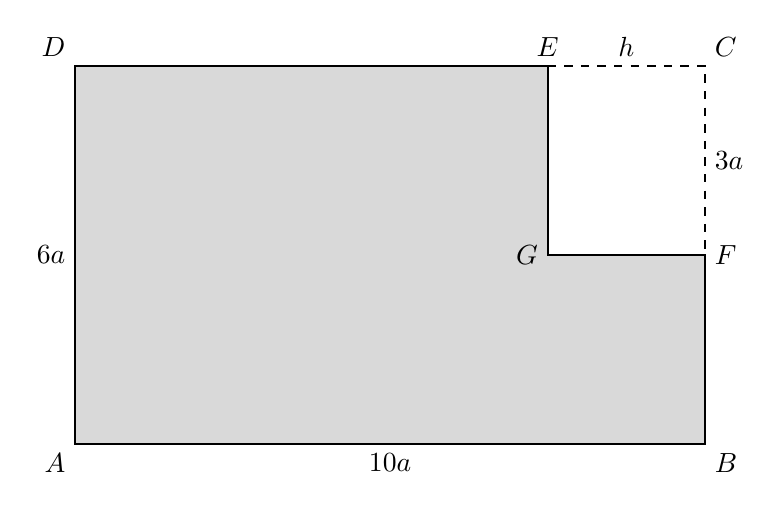
\begin{tikzpicture}[scale=0.8]
\def\W{10}
\def\H{6}
\def\k{3}
\def\h{2.5}
\coordinate (A) at (0,0);
\coordinate (B) at (\W,0);
\coordinate (C) at (\W,\H);
\coordinate (D) at (0,\H);
\coordinate (E) at ({\W-\h},\H);
\coordinate (F) at (\W,{\H-\k});
\coordinate (G) at ({\W-\h},{\H-\k});

\fill[gray!30] (A) -- (B) -- (F) -- (G) -- (E) -- (D) -- cycle;
\draw[thick] (A) -- (B) -- (F) -- (G) -- (E) -- (D) -- cycle;
\draw[dashed, thick] (E) -- (C) -- (F);

\node[below left] at (A) {$A$};
\node[below right] at (B) {$B$};
\node[above right] at (C) {$C$};
\node[above left] at (D) {$D$};
\node[above] at (E) {$E$};
\node[right] at (F) {$F$};
\node[left] at (G) {$G$};

\node[above] at ($(E)!0.5!(C)$) {$h$};
\node[right] at ($(C)!0.5!(F)$) {$3a$};
\node[below] at ($(A)!0.5!(B)$) {$10a$};
\node[left] at ($(A)!0.5!(D)$) {$6a$};
\end{tikzpicture}
\end{figure}


$ABCD$ is a uniform rectangular lamina with $AB=10a$ and $BC=6a$. Point $E$ lies on $DC$ with $CE=h$, where $0<h<10a$, and point $F$ lies on $BC$ with $CF=3a$. The rectangle $CEGF$ is removed, where $G$ is the fourth vertex of the rectangle (see diagram). \\
\begin{enumerate}[label=\textbf{(\alph*)}]
  \item Show that the distance of the centre of mass of the remaining lamina from $AD$ is
  \[
  \dfrac{h^2-20ah+200a^2}{2(20a-h)}
  \]
  and find a corresponding expression for the distance of the centre of mass from $AB$. \marks{5} \\
\end{enumerate}
When the lamina is suspended from the point $D$, the edge $DA$ makes an angle $\theta$ with the downward vertical, where $\tan\theta=\tfrac{13}{12}$. \\
\begin{enumerate}[label=\textbf{(\alph*)}, resume]
  \item Find, in terms of $a$, the two possible values of $h$. \marks{3} \\
\end{enumerate}

\vspace*{10pt}

\begin{tcolorbox}[colback=white, colframe=scarlet, title={\textbf{Solution}}, breakable, grow to left by=6mm, grow to right by=10mm]
\begin{enumerate}[label=\textbf{(\alph*)}, start=1]
  \item Take $A$ as the origin, with $AB$ as the $x$-axis and $AD$ as the $y$-axis.

  Then the whole rectangle $ABCD$ has area
  \[
  60a^2
  \]
  and centre $(5a,3a)$.

  The removed rectangle $CEGF$ has width $h$ and height $3a$, so its area is
  \[
  3ah
  \]
  and its centre is
  \[
  \left(10a-\frac{h}{2},\frac{9a}{2}\right)
  \]

  Because the density is constant and the material is the same, areas can be used as weights.

  So the area of the remaining lamina is
  \[
  60a^2-3ah=3a(20a-h)
  \]

  If the centre of mass of the remaining lamina is $(\bar x,\bar y)$, then
  \[
  (60a^2-3ah)\bar x=60a^2(5a)-3ah\left(10a-\frac{h}{2}\right)
  \]

  Hence
  \begin{align*}
  3a(20a-h)\bar x
  &=300a^3-30a^2h+\frac{3}{2}ah^2 \\
  \bar x
  &=\frac{300a^3-30a^2h+\frac{3}{2}ah^2}{3a(20a-h)} \\
  &=\frac{100a^2-10ah+\frac{1}{2}h^2}{20a-h} \\
  &=\frac{h^2-20ah+200a^2}{2(20a-h)}
  \end{align*}

  So the distance from $AD$ is
  \[
  \frac{h^2-20ah+200a^2}{2(20a-h)}
  \]

  Similarly,
  \[
  (60a^2-3ah)\bar y=60a^2(3a)-3ah\left(\frac{9a}{2}\right)
  \]

  So
  \begin{align*}
  3a(20a-h)\bar y
  &=180a^3-\frac{27}{2}a^2h \\
  \bar y
  &=\frac{180a^3-\frac{27}{2}a^2h}{3a(20a-h)} \\
  &=\frac{120a^2-9ah}{2(20a-h)} \\
  &=\frac{3a(40a-3h)}{2(20a-h)}
  \end{align*}

  Therefore the corresponding distance from $AB$ is
  \[
  \frac{3a(40a-3h)}{2(20a-h)}
  \]

  \item When the lamina is suspended from $D$, the centre of mass lies vertically below $D$.

  From part (a), the horizontal distance of the centre of mass from $D$ is $\bar x$, and the vertical distance below $D$ is
  \begin{align*}
  6a-\bar y
  &=6a-\frac{3a(40a-3h)}{2(20a-h)} \\
  &=\frac{12a(20a-h)-3a(40a-3h)}{2(20a-h)} \\
  &=\frac{3a(40a-h)}{2(20a-h)}
  \end{align*}

  Hence
  \[
  \tan\theta=\frac{\bar x}{6a-\bar y}=\frac{13}{12}
  \]

  Substituting the expressions from part (a):
  \begin{align*}
  \frac{\dfrac{h^2-20ah+200a^2}{2(20a-h)}}{\dfrac{3a(40a-h)}{2(20a-h)}}
  &=\frac{13}{12} \\
  \frac{h^2-20ah+200a^2}{3a(40a-h)}
  &=\frac{13}{12}
  \end{align*}

  So
  \begin{align*}
  12(h^2-20ah+200a^2)&=39a(40a-h) \\
  12h^2-240ah+2400a^2&=1560a^2-39ah \\
  12h^2-201ah+840a^2&=0
  \end{align*}

  Solving this quadratic for $h$:
  \begin{align*}
  h
  &=\frac{201a\pm\sqrt{201^2a^2-4(12)(840)a^2}}{24} \\
  &=\frac{201a\pm 9a}{24}
  \end{align*}

  Hence
  \[
  h=8a \quad \text{or} \quad h=\frac{35a}{4}
  \]

  Both values satisfy $0<h<10a$.
\end{enumerate}
\end{tcolorbox}


\newpage

% ---- Question 9 ----
\questionitem
% [Source: _QBT___Solns__Centre_of_Mass_of_Polygonal_Laminae, Q9]

\begin{figure}[H]
    \centering
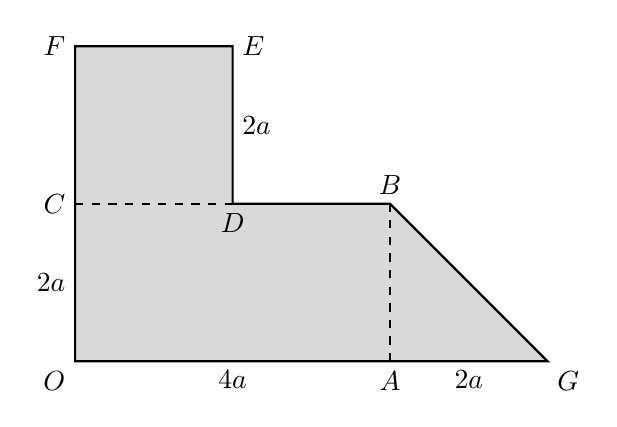
\begin{tikzpicture}[scale=1.0]
\def\w{4}
\def\h{2}
\def\s{2}

\coordinate (O) at (0,0);
\coordinate (A) at (\w,0);
\coordinate (G) at ({\w+\s},0);
\coordinate (B) at (\w,\h);
\coordinate (C) at (0,\h);
\coordinate (D) at (\s,\h);
\coordinate (E) at (\s,{\h+\s});
\coordinate (F) at (0,{\h+\s});

\fill[gray!30] (O) -- (A) -- (B) -- (C) -- cycle;
\fill[gray!30] (C) -- (D) -- (E) -- (F) -- cycle;
\fill[gray!30] (A) -- (G) -- (B) -- cycle;

\draw[thick] (O) -- (A) -- (G) -- (B) -- (D) -- (E) -- (F) -- (C) -- cycle;

\draw[dashed, thick] (A) -- (B);
\draw[dashed, thick] (C) -- (D);

\node[below] at ($(O)!0.5!(A)$) {$4a$};
\node[below] at ($(A)!0.5!(G)$) {$2a$};
\node[left] at ($(O)!0.5!(C)$) {$2a$};
\node[right] at ($(D)!0.5!(E)$) {$2a$};

\node[below left] at (O) {$O$};
\node[below] at (A) {$A$};
\node[below right] at (G) {$G$};
\node[above] at (B) {$B$};
\node[left] at (C) {$C$};
\node[below] at (D) {$D$};
\node[right] at (E) {$E$};
\node[left] at (F) {$F$};
\end{tikzpicture}
\end{figure}


The uniform plane lamina shown in the diagram is formed from the rectangle $OABC$, the square $CDEF$ and the triangle $ABG$. The rectangle has dimensions $4a$ by $2a$, the square has side $2a$ and $AG=2a$. Take $O$ as the origin, with $OA$ as the positive $x$-axis and $OC$ as the positive $y$-axis. \\

In part (a) you may use, without proof, any of the centre of mass formulae given in the formulae booklet. \\
\begin{enumerate}[label=\textbf{(\alph*)}]
  \item Show that the distance of the centre of mass of triangle $ABG$ from $AB$ is $\dfrac{2a}{3}$. \marks{3} \\
  \item Find the coordinates of the centre of mass of the lamina. \marks{4} \\
\end{enumerate}
The lamina is freely suspended from $F$ and hangs in equilibrium with $FC$ at an angle $\theta^\circ$ to the downward vertical. \\
\begin{enumerate}[label=\textbf{(\alph*)}, resume]
  \item Find the value of $\theta$. \marks{4} \\
\end{enumerate}

\vspace*{10pt}

\begin{tcolorbox}[colback=white, colframe=scarlet, title={\textbf{Solution}}, breakable, grow to left by=6mm, grow to right by=10mm]
\begin{enumerate}[label=\textbf{(\alph*)}, start=1]
  \item Let the centre of mass of triangle $ABG$ be $T$.

For a triangular lamina, the centroid has coordinates equal to the mean of the coordinates of its vertices.

\[
T=\left(\frac{4a+4a+6a}{3},\frac{0+2a+0}{3}\right)=\left(\frac{14a}{3},\frac{2a}{3}\right)
\]

The line $AB$ is vertical, with equation $x=4a$.
So the perpendicular distance of $T$ from $AB$ is

\[
\frac{14a}{3}-4a=\frac{14a-12a}{3}=\frac{2a}{3}
\]

Hence the distance of the centre of mass of triangle $ABG$ from $AB$ is $\dfrac{2a}{3}$.

  \item Let the centre of mass of the whole lamina be $(\bar{x},\bar{y})$.

Because the density is constant and the materials are the same, areas can be used as weights.

For the three parts:
\[
\begingroup
\renewcommand{\arraystretch}{2.0}
\begin{array}{c|c|c}
\text{Shape} & \text{Area} & \text{Centre of mass} \\
\hline
\text{Rectangle }OABC & 8a^2 & (2a,a) \\
\text{Square }CDEF & 4a^2 & (a,3a) \\
\text{Triangle }ABG & 2a^2 & \left(\dfrac{14a}{3},\dfrac{2a}{3}\right)
\end{array}
\endgroup
\]

So the total area is

\[
8a^2+4a^2+2a^2=14a^2
\]

Using $A\bar{x}=A_1x_1+A_2x_2+A_3x_3$,

\begin{align*}
14a^2\bar{x} &= 8a^2(2a)+4a^2(a)+2a^2\left(\frac{14a}{3}\right) \\
&= 16a^3+4a^3+\frac{28a^3}{3} \\
&= \frac{88a^3}{3}
\end{align*}

Hence

\[
\bar{x}=\frac{88a^3/3}{14a^2}=\frac{44a}{21}
\]

Using $A\bar{y}=A_1y_1+A_2y_2+A_3y_3$,

\begin{align*}
14a^2\bar{y} &= 8a^2(a)+4a^2(3a)+2a^2\left(\frac{2a}{3}\right) \\
&= 8a^3+12a^3+\frac{4a^3}{3} \\
&= \frac{64a^3}{3}
\end{align*}

Hence

\[
\bar{y}=\frac{64a^3/3}{14a^2}=\frac{32a}{21}
\]

So the coordinates of the centre of mass of the lamina are

\[
\left(\frac{44a}{21},\frac{32a}{21}\right)
\]

  \item Let the centre of mass be $M$.

When the lamina is freely suspended from $F$, the centre of mass lies vertically below $F$ in equilibrium.
So the downward vertical is along the line $FM$.

Now

\[
F=(0,4a), \qquad M=\left(\frac{44a}{21},\frac{32a}{21}\right)
\]

Hence

\[
\overrightarrow{FM}=\left(\frac{44a}{21},\frac{32a}{21}-4a\right)=\left(\frac{44a}{21},-\frac{52a}{21}\right)
\]

The line $FC$ is vertical in the lamina, so after turning through angle $\theta$, it makes angle $\theta$ with the downward vertical.
Therefore $\theta$ is the angle between $FC$ and $FM$.

Using the horizontal and vertical components of $FM$,

\[
\tan\theta=\frac{44a/21}{52a/21}=\frac{11}{13}
\]

So

\[
\theta=\arctan\left(\frac{11}{13}\right)\approx 40.2^\circ
\]

Hence the value of $\theta$ is $\arctan\!\left(\dfrac{11}{13}\right)$, which is approximately $40.2^\circ$.
\end{enumerate}
\end{tcolorbox}


\newpage

% ---- Question 10 ----
\questionitem
% [Source: _QBT___Solns__Centre_of_Mass_of_Polygonal_Laminae, Q10]

\begin{figure}[H]
    \centering
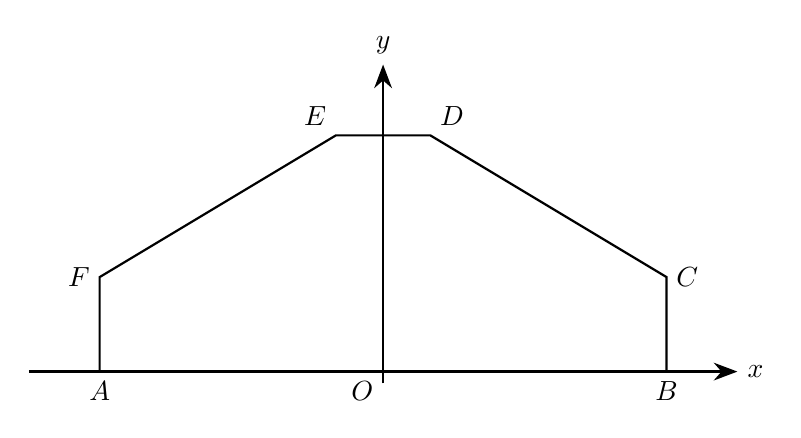
\begin{tikzpicture}[x=0.03cm,y=0.03cm]
\coordinate (O) at (0,0);
\coordinate (A) at (-120,0);
\coordinate (B) at (120,0);
\coordinate (C) at (120,40);
\coordinate (D) at (20,100);
\coordinate (E) at (-20,100);
\coordinate (F) at (-120,40);
\coordinate (X) at (150,0);
\coordinate (Y) at (0,130);

\draw[-{Stealth[length=3mm]}, thick] (-150,0) -- (X) node[right] {$x$};
\draw[-{Stealth[length=3mm]}, thick] (0,-5) -- (Y) node[above] {$y$};
\draw[thick] (A) -- (B) -- (C) -- (D) -- (E) -- (F) -- cycle;

\node[below] at (A) {$A$};
\node[below] at (B) {$B$};
\node[right] at (C) {$C$};
\node[above right] at (D) {$D$};
\node[above left] at (E) {$E$};
\node[left] at (F) {$F$};
\node[below left] at (O) {$O$};
\end{tikzpicture}
\end{figure}


A uniform lamina $ABCDEF$ is in the shape of the hexagon shown in the diagram. In a coordinate system with origin $O$, the vertices have coordinates $A(-120,0)$, $B(120,0)$, $C(120,40)$, $D(20,100)$, $E(-20,100)$ and $F(-120,40)$. The units of the axes are centimetres. \\

The centre of mass of the lamina lies at $(\bar{x},\bar{y})$. \\
\begin{enumerate}[label=\textbf{(\alph*)}]
  \item Use symmetry to write down $\bar{x}$ and show that $\bar{y}=40$. \marks{5} \\
\end{enumerate}
The lamina is placed horizontally so that it rests on three supports, whose points of contact are at $D$, $E$ and $G$, where $G$ lies on the edge $AB$ and has coordinates $(g,0)$. \\
\begin{enumerate}[label=\textbf{(\alph*)}, resume]
  \item Determine the range of values of $g$ for the lamina to rest in equilibrium. \marks{3} \\
\end{enumerate}
It is now given that $g=8$, and that the lamina has weight $100\mathrm{N}$. \\
\begin{enumerate}[label=\textbf{(\alph*)}, resume]
  \item Determine the forces exerted on the lamina by each of the supports at $D$, $E$ and $G$. \marks{4} \\
\end{enumerate}

\vspace*{10pt}

\begin{tcolorbox}[colback=white, colframe=scarlet, title={\textbf{Solution}}, breakable, grow to left by=6mm, grow to right by=10mm]
\begin{enumerate}[label=\textbf{(\alph*)}, start=1]
\item The hexagon is symmetric about the \(y\)-axis, so
\[
\bar{x}=0
\]

To find \(\bar{y}\), take the lamina as a \(240\times 100\) rectangle with two identical right-angled triangles removed.

Because the density is constant and the material is the same, areas can be used as weights.

For the rectangle,
\[
A_1=240\times 100=24000,
\qquad y_1=50
\]

For each removed triangle,
\[
A_2=\frac12\times 100\times 60=3000
\]
and its centroid is \(\frac13\) of the height down from the top edge \(y=100\), so
\[
y_2=100-\frac{60}{3}=80
\]

Hence the area of the hexagon is
\[
A=24000-2(3000)=18000
\]

Now take moments about the \(x\)-axis:
\[
A\bar{y}=A_1y_1-2A_2y_2
\]
so
\begin{align*}
18000\bar{y}
&=24000(50)-2(3000)(80)\\
&=1200000-480000\\
&=720000
\end{align*}

Therefore
\[
\bar{y}=\frac{720000}{18000}=40
\]

So the centre of mass is
\[
(\bar{x},\bar{y})=(0,40)
\]

\item For the lamina to rest in equilibrium, the vertical line through the centre of mass must pass inside or on the triangle formed by the three supports, that is triangle \(DEG\).

From part (a), the centre of mass is at \((0,40)\). So we need the point \((0,40)\) to lie inside or on triangle \(DEG\).

First find where the line \(DG\) has height \(y=40\). Using coordinates \(D(20,100)\) and \(G(g,0)\),
\[
\frac{40-0}{100-0}=\frac{x-g}{20-g}
\]
Hence
\begin{align*}
\frac{2}{5}&=\frac{x-g}{20-g}\\
x-g&=\frac{2}{5}(20-g)\\
x&=8+\frac{3g}{5}
\end{align*}

Now do the same for line \(EG\), where \(E(-20,100)\):
\[
\frac{40-0}{100-0}=\frac{x-g}{-20-g}
\]
Hence
\begin{align*}
\frac{2}{5}&=\frac{x-g}{-20-g}\\
x-g&=\frac{2}{5}(-20-g)\\
x&=-8+\frac{3g}{5}
\end{align*}

So at height \(y=40\), triangle \(DEG\) runs from
\[
x=-8+\frac{3g}{5}
\quad \text{to} \quad
x=8+\frac{3g}{5}
\]

For \((0,40)\) to lie on or between these values,
\[
-8+\frac{3g}{5}\le 0 \le 8+\frac{3g}{5}
\]

This gives
\[
g\le \frac{40}{3}
\qquad \text{and} \qquad
g\ge -\frac{40}{3}
\]

Therefore the required range is
\[
-\frac{40}{3}\le g\le \frac{40}{3}
\]

\item Let the upward support forces at \(D\), \(E\) and \(G\) be \(R_D\), \(R_E\) and \(R_G\) respectively.

Since the lamina is in equilibrium, the resultant of these three upward forces is equal to the weight \(100\,\mathrm{N}\), and it acts through the centre of mass \((0,40)\).

So
\[
R_D+R_E+R_G=100
\]

Using the \(y\)-coordinates of the supports,
\[
100\times 40=100R_D+100R_E+0\cdot R_G
\]
so
\[
R_D+R_E=40
\]

Hence
\[
R_G=100-40=60
\]

Now use the \(x\)-coordinates of the supports. Since the resultant acts through \(x=0\),
\[
100\times 0=20R_D+(-20)R_E+8R_G
\]
So
\begin{align*}
20R_D-20R_E+8(60)&=0\\
20R_D-20R_E&=-480\\
R_D-R_E&=-24
\end{align*}

Now solve
\[
R_D+R_E=40,
\qquad
R_D-R_E=-24
\]

Adding gives
\[
2R_D=16
\]
so
\[
R_D=8
\]
and then
\[
R_E=32
\]

Therefore the forces exerted on the lamina are:
\[
\text{at }D:\ 8\,\mathrm{N}\text{ upward},\qquad
\text{at }E:\ 32\,\mathrm{N}\text{ upward},\qquad
\text{at }G:\ 60\,\mathrm{N}\text{ upward}
\]
\end{enumerate}
\end{tcolorbox}


\end{enumerate}
\end{document}
